\section{Materialien}

Auf der Veranstaltungsseite stellen wir Ihnen einige Dateien zur Verf\"ugung, die Sie f\"ur Ihre L\"osung verwenden k\"onnen. Dabei handelt es sich um vorgefertigte Karten und
die \"offentlichen Testf\"alle. Es wird Ihnen dringend nahe gelegt, auch unser bereitgestelltes Framework nutzen. Das Framework ist threadsicher!

\textbf{Hinweis:} Sie dürfen auch eine vollst\"andig eigene L\"osungen implementieren. Der dadurch entstehende Mehraufwand wird aber nicht durch Punkte gewürdigt. Ihre L\"osung \textbf{muss} in jedem Fall mit den bereitgestellten Testklassen \"uberpr\"ufbar sein.

Neben der kurzen Beschreibung in diesem Dokument gibt Ihnen die
JavaDoc-Dokumentation n\"utzliche Hinweise zur Verwendung und den
Parametern der vorhandenen Funktionen. Ein Blick in diese Quellen empfiehlt sich
sehr---\textbf{am besten vor dem Gang zum\_zur Tutor\_in}, um$\ldots$

\begin{itemize}
\item sich selbst und auch dem\_der Tutor\_in wertvolle Zeit zu sparen, da sich so unter Umst\"anden banale Fragen von selbst l\"osen,

\item Nerven zu sparen, da das Warten auf die Antwort der Tutor\_innen Ihre Nerven beanspruchen wird :-),

\item sich selbstst\"andiges Arbeiten anzueignen.
\end{itemize} 


\subsection{Klasse \emph{de.tu\_darmstadt.informatik.fop.gorillas.main.Gorillas}}

\textit{\gameTitle} erbt von \textit{org.slick.StateBasedGame}. \textit{\gameTitle} dient sowohl als Container für Spiele 
als auch zum Starten des gesamten Spiels. Sie müssen diese Klasse erweitern, um zusätzliche States hinzuzufügen. Lesen Sie sich dazu das \tutorialURL durch.

\subsection {Die ersten Schritte}
Sie sollten sich zunächst das  \tutorialURL 
durchlesen, um das Konzept des Frameworks zu verstehen. Anschließend können Sie in \texttt{\gameTitle} zusätzliche 
States (Fenster) definieren. Sie sollten mit einem Hauptmenü und einem Spielfenster beginnen.

Anschließend sollten Sie in der Gruppe diskutieren, wie Ihr Projekt strukturiert werden soll und Aufgaben in der Gruppe verteilen.

% basicevents
\subsection {Basisereignisse und Basisaktionen}

Das \textbf{eea}-Framework arbeitet mit \textbf{Entit\"aten}, wie der \textbf{ImageRenderComponent}, sowie \textbf{Events} und
zugehörigen \textbf{Actions}. Die zwei Tabellen am Ende geben einen Überblick über die mitgelieferten Events und Actions.
Das Neuzeichnen eines Fensters geschieht zusammen mit einem Frame.

\begin{table}[htbp]
\begin{tabular}{|p{.45\textwidth}|p{.5\textwidth}|}\hline

\textbf{Konstruktor} & \textbf{Beschreibung}\\\hline\hline
\emph{CollisionEvent()} & Dieses Event wird (mit jedem Frame) ausgelöst, wenn sich zwei Entitäten überlappen.\\\hline
\emph{KeyPressedEvent(String id, Integer... key)} & Dieses Event wird ausgelöst, wenn die Taste gerade erstmalig nach unten gedrückt wurde.\\\hline
\emph{KeyDownEvent(String id, Integer... key)} & Dieses Event wird ausgelöst, wenn die Taste aktuell unten gehalten wird.\\\hline
\emph{LeavingScreenEvent()} & Dieses Event wird ausgelöst, wenn die an diesem Event interessierte Entität die Spielfl\"ache verlassen hat.\\\hline
\emph{LoopEvent(String id)} & Dieses Event wird mit jedem Frame ausgelöst. Dieses Event eignet sich also dafür, in jedem Frame eine gewisse Aktion auszuführen.\\\hline
\emph{MouseClickedEvent()} & Dieses Event wird ausgelöst, wenn die Maus auf die an dem Event interessierte Entität geklickt hat.\\\hline
\emph{MouseEnteredEvent()} & Dieses Event wird ausgelöst, wenn die Maus über die an dem Event interessierte Entität fährt.\\\hline
\emph{MovementDoesntCollideEvent(float speed, IMovement move)} & Dieses Event wird ausgelöst, wenn die Bewegung (Action) keine Kollision mit einer anderen Entität verursacht.\\\hline

\end{tabular}
\caption{Basisereignisse des \textbf{eea}-Frameworks aus dem package \emph{eea.engine.events.basicevents}}
\end{table}

% basicevents
%\subsection {Basisaktionen}

\begin{table}[htbp]
\begin{tabular}{|p{.4\textwidth}|p{.5\textwidth}|}\hline
\textbf{Konstruktor} & \textbf{Beschreibung}\\\hline\hline
\emph{ChangeStateAction(int state)} & Diese Action wechselt in einen Zustand (State) mit der State-ID \textbf{state}. Ist der State schon einmal initialisiert worden, so wird die \textbf{init}-Methode nicht erneut aufgerufen.\\\hline
\emph{ChangeStateInitAction(int state)} & Diese Action wechselt in einen State mit der State-ID state. Auch wenn der State schon einmal initialisiert worden ist, 
wird die \textbf{init}-Methode erneut aufgerufen.\\\hline
\emph{DestroyEntityAction()} & Diese Action zerstört die Entität bei Eintreten eines gewissen Events.\\\hline
\emph{MoveBackwardAction(float speed)*} & Diese Action führt mit einer Geschwindigkeit \textbf{speed} eine Rückwärtsbewegung entgegen der Blickrichtung aus.\\\hline
\emph{MoveDownAction(float speed()*} & Diese Action führt mit einer Geschwindigkeit \textbf{speed} eine Bewegung nach unten aus.\\\hline
\emph{MoveForwardAction(float speed)*} & Diese Action führt mit einer Geschwindigkeit \textbf{speed} eine Vorwärtsbewegung in Blickrichtung aus.\\\hline
\emph{MoveLeftAction(float speed)*} & Diese Action führt mit einer Geschwindigkeit \textbf{speed} eine Bewegung nach links aus.\\\hline
\emph{MoveRightAction(float speed)*} & Diese Action führt mit einer Geschwindigkeit \textbf{speed} eine Bewegung nach rechts aus.\\\hline
\emph{MoveUpAction(float speed)*} & Diese Action führt mit einer Geschwindigkeit \textbf{speed} eine Bewegung nach oben aus.\\\hline
\emph{RotateLeftAction(float speed)*} & Diese Action führt mit einer Geschwindigkeit \textbf{speed} eine Drehung nach links aus.\\\hline
\emph{RotateRightAction(float speed)*} & Diese Action führt mit einer Geschwindigkeit \textbf{speed} eine Drehung nach rechts aus.\\\hline
\emph{QuitAction()} & Diese Action beendet das laufende Spiel.\\\hline
\emph{RemoveEventAction()} & Diese Action zerstört ein Event.\\\hline
\emph{SetEntityPositionAction(Vector2f pos)} & Diese Action setzt die Position einer Entität neu.\\\hline

\end{tabular}
\caption{Basisaktionen des \textbf{eea}-Frameworks aus dem package \emph{eea.engine.actions.basicactions.} Die mit einem * markierten Aktionen sind für das Spiel \gameTitle nicht von Bedeutung. Um den Wurf eines Objektes zu simulieren, empfiehlt es sich eine eigene MoveAction zu implementieren. Die Richtungen werden verdeutlicht durch Abbildung \vref{fig:screenshot3}.}
\end{table}

\begin{figure}[htbp]
\begin{center}
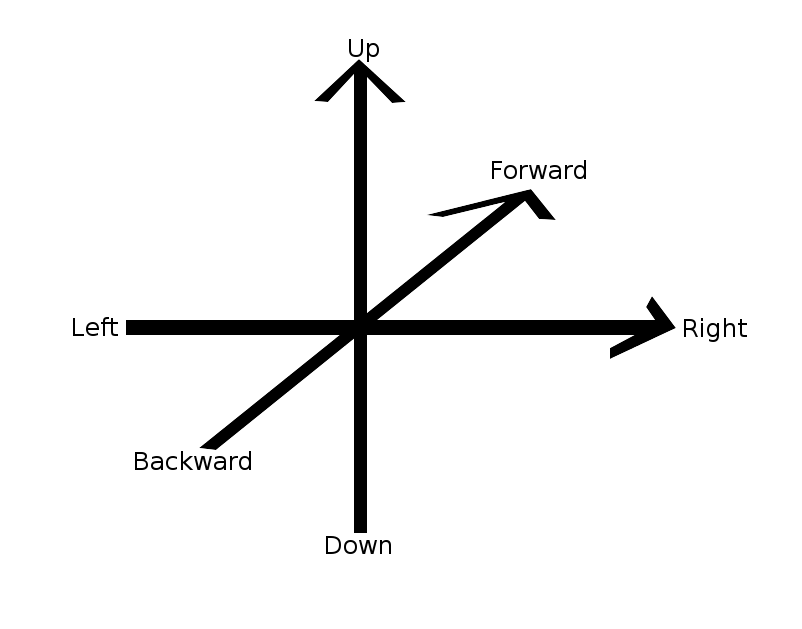
\includegraphics[width=7cm]{\basepath/\shortGameTitle/directions.png}
\caption{Es gibt zahlreiche Aktionen, die eine Bewegung ausdrücken.}
\label{fig:screenshot3}
\end{center}
\end{figure}
